\documentclass[pre,aps,superscriptaddress,nofootinbib]{revtex4}

\usepackage{amsmath,amsfonts,amssymb,bm,graphicx,hyperref,listings,xcolor,float}
\setlength{\parindent}{0pt}

\begin{document}

\title{2 RTPs on a ring}
\author{Yann-Edwin Keta}
\maketitle

% \maketitle

\nocite{slowman2016jamming}

\section{Model}

\subsection{Fokker-Planck equations}

We consider 2 run-and-tumble particles (RTPs), with swim speed $v_0$ and tumble rate $\tau^{-1}$ on a linear ring of length $L$. With $r_1, r_2 \in [0, L]$ the positions and $\alpha_1, \alpha_2 = \pm$ the states of each particles, and $V(r_1, r_2) = V(|r_1 - r_2|)$ the potential of interactions between these particles, we have the equations of motion
\begin{equation}
\dot{r}_i = \alpha_i v_0 - \partial_{r_i} V(|r_1 - r_2|)
\label{EOM}
\end{equation}
and the Fokker-Planck equations for the joint distribution of positions
\begin{equation}
\begin{aligned}
\dot{P}_{\alpha_1, \alpha_2}(r_1, r_2) =
  &- v_0(\alpha_1 \partial_{r_1} + \alpha_2 \partial_{r_2}) P_{\alpha_1\alpha_2}(r_1, r_2)
    &&\to \text{Propulsion}\\
  &+ \partial_{r_1} (P_{\alpha_1\alpha_2}(r_1, r_2)\partial_{r_1}V(|r_1 - r_2|))
    &&\to \text{Interaction}\\
  &+ \partial_{r_2} (P_{\alpha_1\alpha_2}(r_1, r_2)\partial_{r_2}V(|r_1 - r_2|))
    &&\\
  &+ \tau^{-1} (P_{\overline{\alpha_1}\alpha_2}(r_1, r_2) + P_{\alpha_1\overline{\alpha_2}}(r_1, r_2) - 2 P_{\alpha_1\alpha_2}(r_1, r_2))
    &&\to \text{Tumble}\\
  =& \, \mathcal{L}^{\dagger}_{\alpha_1\alpha_2} P_{\alpha_1\alpha_2}(r_1, r_2)
\end{aligned}
\label{FP0}
\end{equation}
with $\mathcal{L}^{\dagger}_{\alpha_1\alpha_2}$ the Fokker-Planck operator.\\

We introduce $r \equiv r_2 - r_1 > 0$, such that $\partial_{r_1} \equiv - \partial_r$ and $\partial_{r_2} = \partial_r$, with which we can define the symmetries
\begin{eqnarray}
\label{evensymmetry}
P_{++}(r) = P_{--}(r),\\
\label{oddsymmetry}
P_{+-}(r) = P_{-+}(L - r),
\end{eqnarray}
and the interaction potential
\begin{align*}
V(r) = \begin{cases} 0 &\text{ if } r \in ]0, L[ \\ \infty &\text{ otherwise} \end{cases}
\end{align*}
such that, with Eq. (\ref{EOM}), we get for particles with opposite directions
\begin{equation}
- \partial_r V(0) = \partial_r V(L) = v_0.
\end{equation}
because of mutual hindrance.\\

We can solve the steady state problem with the normalisation condition
\begin{equation}
\int_0^L \mathrm{d}r \, \sum_{\alpha_1\alpha_2} P_{\alpha_1\alpha_2}(r) = 1
\label{normalisation}
\end{equation}
the bulk equations
\begin{equation}
\dot{P}_{\alpha_1\alpha_2}(r \in ]0, L[) = 0
\label{bulk}
\end{equation}
the left boundary equations
\begin{equation}
\int_{0^-}^{0^+} \mathrm{d}r \, \dot{P}_{\alpha_1\alpha_2}(r) = 0
\label{leftboundary}
\end{equation}
and the right boundary equations
\begin{equation}
\int_{L^-}^{L^+} \mathrm{d}r \, \dot{P}_{\alpha_1\alpha_2}(r) = 0.
\label{rightboundary}
\end{equation}

\subsection{Biased ensemble}

We define our biasing quantity
\begin{equation}
\dot{Z} = \sum_{i=1}^2 - \partial_r V(r) \alpha_i v_0 = v_0 (\alpha_1 - \alpha_2) \partial_r V(r)
\end{equation}
which is non-zero only at contact, and the tilted generator
\begin{equation}
\mathcal{W}^{\dagger}_{\alpha_1\alpha_2} = \mathcal{L}^{\dagger}_{\alpha_1\alpha_2} - s \dot{Z}
\end{equation}
with $s$ the biasing parameter, which eigenvalue problem
\begin{equation}
\psi P_{\alpha_1\alpha_2}(r) = \mathcal{W}^{\dagger}_{\alpha_1\alpha_2} P_{\alpha_1\alpha_2}(r)
\label{eigenproblem}
\end{equation}
we have to solve for $\psi(s)$ its largest eigenvalue, which defines the dynamical free energy.\\

While the symmetries (Eqs. (\ref{evensymmetry}, \ref{oddsymmetry})) and the normalisation condition (Eq. (\ref{normalisation})) remains unchanged, we have that the bulk equations (Eq. (\ref{bulk})), the left boundary equations (Eq. \ref{leftboundary}), and the right boundary equations (Eq. \ref{rightboundary}) become
\begin{eqnarray}
\label{bulk:biased}
\psi P_{\alpha_1\alpha_2}(r \in ]0, L[) = \mathcal{W}^{\dagger}_{\alpha_1\alpha_2} P_{\alpha_1\alpha_2}(r \in ]0, L[)\\
\label{leftboundary:biased}
\int_{0^-}^{0^+} \mathrm{d}r \, \psi P_{\alpha_1\alpha_2}(r) = \int_{0^-}^{0^+} \mathrm{d}r \, \mathcal{W}^{\dagger}_{\alpha_1\alpha_2} P_{\alpha_1\alpha_2}(r)\\
\label{rightboundary:biased}
\int_{L^-}^{L^+} \mathrm{d}r \, \psi P_{\alpha_1\alpha_2}(r) = \int_{L^-}^{L^+} \mathrm{d}r \, \mathcal{W}^{\dagger}_{\alpha_1\alpha_2} P_{\alpha_1\alpha_2}(r)
\end{eqnarray}
respectively.

\section{Unbiased steady state distribution}

We use the following ansatz for the unbiased ($s = 0$) steady state distribution
\begin{equation}
P_{\alpha_1\alpha_2}(r) = a_{\alpha_1\alpha_2} + b_{\alpha_1\alpha_2} \delta(r) + c_{\alpha_1\alpha_2} \delta(L - r)
\end{equation}
which satisfies the normalisation condition (Eq. (\ref{normalisation}))
\begin{equation}
\sum_{\alpha_1\alpha_2} \left(L a_{\alpha_1\alpha_2} + b_{\alpha_1\alpha_2} + c_{\alpha_1\alpha_2}\right) = 1
\end{equation}
the bulk equations (Eq. (\ref{bulk}))
\begin{eqnarray}
\tau^{-1} (a_{+-} + a_{-+} - 2 a_{++}) = 0\\
\tau^{-1} (a_{+-} + a_{-+} - 2 a_{--}) = 0\\
\tau^{-1} (a_{++} + a_{--} - 2 a_{+-}) = 0\\
\tau^{-1} (a_{++} + a_{--} - 2 a_{-+}) = 0
\end{eqnarray}
the left boundary equations (Eq. (\ref{leftboundary}))
\begin{eqnarray}
\tau^{-1}(b_{+-} + b_{-+} - 2 b_{++}) = 0\\
\tau^{-1}(b_{+-} + b_{-+} - 2 b_{--}) = 0\\
2 v_0 a + \tau^{-1}(b_{++} + b_{--} - 2 b_{+-}) = 0\\
- 2 v_0 a + \tau^{-1}(b_{++} + b_{--} - 2 b_{-+}) = 0
\end{eqnarray}
the right boundary equations (Eq. (\ref{rightboundary}))
\begin{eqnarray}
\tau^{-1}(c_{+-} + c_{-+} - 2 c_{++}) = 0\\
\tau^{-1}(c_{+-} + c_{-+} - 2 c_{--}) = 0\\
- 2 v_0 a + \tau^{-1}(c_{++} + c_{--} - 2 c_{+-}) = 0\\
2 v_0 a + \tau^{-1}(c_{++} + c_{--} - 2 c_{-+}) = 0
\end{eqnarray}
and the symmetries (Eqs. (\ref{evensymmetry}, \ref{oddsymmetry})).\\

We get
\begin{eqnarray}
P_{++}(r) = a + l a \delta(r) + l a \delta(L - r)\\
P_{--}(r) = a + l a \delta(r) + l a \delta(L - r)\\
P_{+-}(r) = a + 2 l a \delta(r)\\
P_{-+}(r) = a + 2 l a \delta(L - r)
\end{eqnarray}
with
\begin{equation}
a = \frac{1}{4(L + 2l)}
\end{equation}
and the persistence length $l = v_0 \tau$.

\section{Biased steady state distribution}

\subsection{Exact solution}

We use the following ans\"atze for the steady state distribution
\begin{eqnarray}
P_{++}(r) = P_{--}(r) = \beta(r) + \gamma_- \delta(r) + \gamma_+ \delta(L - r)\\
P_{+-}(r) = \varepsilon(r) + \zeta \delta(r)\\
P_{-+}(r) = \theta(r) + \zeta \delta(L - r)\\
\end{eqnarray}
with $\varepsilon(r) = \theta(L - r)$ according to Eq. (\ref{oddsymmetry}).\\

We write the eigenvalue equations (Eq. (\ref{eigenproblem}))
\begin{eqnarray}
\label{FP1}
\psi P_{\alpha\alpha}(r) = 2 \partial_r(P_{\alpha\alpha}(r) \partial_r V(r)) + \tau^{-1} (P_{+-}(r) + P_{-+}(r) - 2 P_{\alpha\alpha}(r))\\
\label{FP2}
\psi P_{+-}(r) = 2 v_0 \partial_r P_{+-}(r) + 2 \partial_r(P_{+-}(r) \partial_r V(r)) + \tau^{-1}(2 P_{\alpha\alpha}(r) - 2 P_{+-}(r)) - 2 s v_0 \partial_r V(r) P_{+-}(r)\\
\label{FP3}
\psi P_{-+}(r) = - 2 v_0 \partial_r P_{-+}(r) + 2 \partial_r(P_{-+}(r) \partial_r V(r)) + \tau^{-1}(2 P_{\alpha\alpha}(r) - 2 P_{-+}(r)) + 2 s v_0 \partial_r V(r) P_{-+}(r)
\end{eqnarray}
and integrate Eq. (\ref{FP3}) between $0^-$ and $L^+$ to get
\begin{equation}
\psi = 2 s v_0 \partial_r V(L) \zeta = 2 s v_0^2 \zeta
\label{psiZeta}
\end{equation}
linking the dynamical free energy $\psi$ and the sticking term $\zeta$.\\

We have the bulk equations (Eq. (\ref{bulk:biased}))
\begin{eqnarray}
\label{bulk:biased1}
\psi \beta(r) = \tau^{-1} (\varepsilon(r) + \theta(r) - 2 \beta(r))\\
\label{bulk:biased2}
\psi \epsilon(r) = 2 v_0 \varepsilon^{\prime}(r) + \tau^{-1} (2 \beta(r) - 2 \varepsilon(r))\\
\label{bulk:biased3}
\psi \theta(r) = -2 v_0 \theta^{\prime}(r) + \tau^{-1} (2 \beta(r) - 2 \theta(r))
\end{eqnarray}
such that Eq. (\ref{bulk:biased1}) gives
\begin{equation}
\beta(r) = (2 + \tau\psi)^{-1} (\epsilon(r) + \theta(r))
\end{equation}
and the difference and sum of Eqs. (\ref{bulk:biased2}, \ref{bulk:biased3}) give
\begin{eqnarray}
2 l (\varepsilon(r) + \theta(r))^{\prime} = (2 \tau + \psi)(\varepsilon(r) - \theta(r))\\
\begin{aligned}
2 l (\varepsilon(r) - \theta(r))^{\prime} &= -4 \beta(r) + (\tau\psi + 2)(\varepsilon(r) + \theta(r))\\
&= \left((\tau\psi + 2) - \frac{4}{\tau\psi + 2}\right)(\varepsilon(r) + \theta(r))
\end{aligned}
\end{eqnarray}
where we set $A(r) = \varepsilon(r) + \theta(r)$ and $B(r) = \varepsilon(r) - \theta(r)$, which on the one hand verify
\begin{equation}
A^{\prime\prime}(r) - k^2 A(r) = 0
\end{equation}
where
\begin{equation}
k^2 l^2 = \frac{\tau \psi}{2}\left(\frac{\tau \psi}{2} + 2\right)
\label{kPsi}
\end{equation}
and which general solution is
\begin{equation}
A(r) = A_+ e^{- k r} + A_- e^{-k (L - r)}
\end{equation}
and on the other hand
\begin{equation}
B(r) = l(1 + \tau \psi/2)^{-1} A^{\prime}(r) = kl (1 + \tau\psi/2)^{-1} (A_- e^{-k(L - r)} - A_+ e^{-k r})
\end{equation}
from which we infer
\begin{eqnarray}
\begin{aligned}
\varepsilon(r) &= \frac{1}{2} (A(r) + B(r))\\
&= \frac{1}{2}\left(1 - k l (1 + \psi \tau/2)^{-1}\right) A_+ e^{- k r} + \frac{1}{2}\left(1 + k l (1 + \psi \tau/2)^{-1}\right) A_- e^{- k (L - r)}
\end{aligned}
\mbox{}\\
\begin{aligned}
\theta(r) &= \frac{1}{2} (A(r) - B(r))\\
&= \frac{1}{2}\left(1 + k l (1 + \psi \tau/2)^{-1}\right) A_+ e^{- k r} + \frac{1}{2}\left(1 - k l (1 + \psi \tau/2)^{-1}\right) A_- e^{- k (L - r)}
\end{aligned}
\end{eqnarray}
where we note that the symmetry condition of Eq. (\ref{oddsymmetry}) implies that $A_- = A_+$, and
\begin{equation}
\begin{aligned}
\beta(r) &= (\tau\psi + 2)^{-1}(\varepsilon(r) + \theta(r)) = (\tau \psi + 2)^{-1} A(r)\\
&= \frac{1}{2}(1 + \tau\psi/2)^{-1}(A_+ e^{-k r} + A_- e^{-k (L - r)})
\end{aligned}
\end{equation}
where we need to determine $A_+ = A_-$.\\

We have the left and right boundary equations (Eqs. (\ref{leftboundary:biased}, \ref{rightboundary:biased})) for $P_{\alpha\alpha}$
\begin{eqnarray}
\psi \gamma_- = \tau^{-1} (\zeta - 2 \gamma_-)\\
\psi \gamma_+ = \tau^{-1} (\zeta - 2 \gamma_+)
\end{eqnarray}
such that
\begin{equation}
\gamma = \gamma_- = \gamma_+ = (\tau \psi + 2)^{-1} \zeta
\end{equation}
which with Eq. (\ref{psiZeta}) gives
\begin{equation}
\psi = 2 s v_0^2 (\tau \psi + 2) \gamma
\label{gammaPsi}
\end{equation}
where we need to determine $\gamma$.\\

We have the left boundary equations (Eq. (\ref{leftboundary:biased})) for $P_{\alpha\overline{\alpha}}$
\begin{eqnarray}
\psi \zeta = 2 v_0 \varepsilon(0^+) + \tau^{-1} (2 \gamma - 2 \zeta) - 2 s v_0 \partial_r V(0) \zeta\\
0 = - 2 v_0 \varepsilon(L^-) + \tau^{-1} 2 \gamma
\end{eqnarray}
from which we get
\begin{eqnarray}
\label{S1}
\left[(\tau\psi + 2)(\tau\psi + 2 - 2 s l v_0) - 2\right] \gamma - l \left(1 - kl  (1 + \tau\psi/2)^{-1}\right) A_+ - l \left(1 + kl(1 + \tau\psi/2)^{-1}\right) e^{-kL} A_- = 0\\
\label{S2}
2 \gamma - l \left(1 - kl (1 + \tau\psi/2)^{-1}\right) e^{-kL} A_+ - l \left(1 + kl (1 + \tau\psi/2)^{-1}\right) A_- = 0
\end{eqnarray}
and the normalisation condition (Eq. (\ref{normalisation}))
\begin{equation}
2((\tau\psi + 2) + 1) \gamma + \frac{1}{k} \left(1 - e^{-kL}\right)\left(1 + (\tau\psi + 2)^{-1}\right) A_+ + \frac{1}{k} \left(1 - e^{-kL}\right)\left(1 + (\tau\psi + 2)^{-1}\right) A_- = 1
\label{S3}
\end{equation}
so we can solve the system of Eqs. (\ref{S1}, \ref{S2}, \ref{S3}) with respect to $\gamma$, $A_+$, $A_-$, or equivalently with $A_+ = A_-$
\begin{eqnarray}
\label{S01}
\left[(\tau\psi + 2)(\tau\psi + 2 - 2 s l v_0) - 2\right] \gamma - l \left[\left(1 - kl  (1 + \tau\psi/2)^{-1}\right) + \left(1 + kl(1 + \tau\psi/2)^{-1}\right) e^{-kL}\right] A_- = 0\\
\label{S02}
2((\tau\psi + 2) + 1) \gamma + \frac{2}{k} \left(1 - e^{-kL}\right)\left(1 + (\tau\psi + 2)^{-1}\right) A_+ = 1
\end{eqnarray}
with respect to $A_+$ and $\gamma$.\\

We use \textsc{SageMath} to solve Eqs. (\ref{S01}, \ref{S02})
\begin{lstlisting}[backgroundcolor=\color{lightgray!20!white}, language=Python, xleftmargin=0.5cm, xrightmargin=0.5cm, framexleftmargin = 0.5em, frame=tlbr,framesep=4pt]
# variables
psi = var('psi')
tau = var('tau')
k = var('k')
L = var('L')
l = var('l')
v0 = var('v0')
s = var('s')

# system [gamma, A]
system = Matrix([

    [(tau*psi + 2)*(tau*psi + 2 - 2 *s*l*v0) - 2,
    -l*((1 - k*l/(1 + (tau*psi)/2)) + (1 + k*l/(1 + (tau*psi)/2))*exp(-k*L))],

    [2*((tau*psi + 2) + 1),
    (2/k)*(1 - exp(-k*L))*(1 + 1/(tau*psi + 2))]

])

# solution
[[gamma], [A]] = system \ Matrix([[0], [1]])
\end{lstlisting}
and get
\begin{eqnarray}
\gamma = \frac{{\left({\left(\frac{2 \, k l}{\psi \tau + 2} + 1\right)} e^{\left(-L k\right)} - \frac{2 \, k l}{\psi \tau + 2} + 1\right)} l}{2 \, {\left({\left(2 \, l s v_{0} - \psi \tau - 2\right)} {\left(\psi \tau + 2\right)} + 2\right)} {\left(\frac{{\left(\psi \tau + 3\right)} {\left({\left(\frac{2 \, k l}{\psi \tau + 2} + 1\right)} e^{\left(-L k\right)} - \frac{2 \, k l}{\psi \tau + 2} + 1\right)} l}{{\left(2 \, l s v_{0} - \psi \tau - 2\right)} {\left(\psi \tau + 2\right)} + 2} + \frac{{\left(\frac{1}{\psi \tau + 2} + 1\right)} {\left(e^{\left(-L k\right)} - 1\right)}}{k}\right)}}\\
A_+ = A_- = -\frac{1}{2 \, {\left(\frac{{\left(\psi \tau + 3\right)} {\left({\left(\frac{2 \, k l}{\psi \tau + 2} + 1\right)} e^{\left(-L k\right)} - \frac{2 \, k l}{\psi \tau + 2} + 1\right)} l}{{\left(2 \, l s v_{0} - \psi \tau - 2\right)} {\left(\psi \tau + 2\right)} + 2} + \frac{{\left(\frac{1}{\psi \tau + 2} + 1\right)} {\left(e^{\left(-L k\right)} - 1\right)}}{k}\right)}}.
\end{eqnarray}

\subsection{Scaling regime}

We assume there exists a scaling form
\begin{equation}
\psi(s) = L^{-2} \Psi(s L)
\end{equation}
so that for $s = \mathcal{O}(L^{-1})$ we have $\psi(s) = \mathcal{O}(L^{-2})$ and $k = \mathcal{O}(L^{-1})$ from Eq. (\ref{kPsi}).\\

We give an expression of Eqs. (\ref{S2}, \ref{S3}) at the lowest order of $L^{-1}$ and using $A_+ = A_-$
\begin{eqnarray}
2 \gamma - (1 + e^{-kL}) A_+ = 0\\
6 \gamma + \frac{6}{2k} (1 - e^{-kL}) A_+ = 1
\end{eqnarray}
from which we infer
\begin{equation}
\gamma = \frac{1}{6} k l \frac{1 + e^{-kL}}{1 - e^{-kL}}
\end{equation}
and an expression of Eq. (\ref{gammaPsi}) at the lowest order of $L^{-1}$
\begin{equation}
\gamma = \frac{\psi}{4 s v_0^2}
\end{equation}
so that with Eq.(\ref{kPsi}) linking $k$ and $\psi$ we get
\begin{eqnarray}
\frac{3}{s L v_0} = \frac{\coth\left(\sqrt{\frac{\psi L^2}{4 l v_0}}\right)}{\sqrt{\frac{\psi L^2}{4 l v_0}}} \Leftrightarrow \frac{1}{\Lambda} = \frac{\coth\left(\sqrt{\Phi}\right)}{\sqrt{\Phi}} &\qquad\qquad s > 0, \psi > 0\\
- \frac{3}{s L v_0} = \frac{\cot\left(\sqrt{\frac{|\psi| L^2}{4 l v_0}}\right)}{\sqrt{\frac{|\psi| L^2}{4 l v_0}}} \Leftrightarrow - \frac{1}{\Lambda} = \frac{\cot\left(\sqrt{|\Phi|}\right)}{\sqrt{|\Phi|}} &\qquad\qquad s < 0, \psi < 0
\end{eqnarray}
where we have set
\begin{eqnarray}
\Lambda = \frac{s L v_0}{3}\\
\Phi = \frac{\psi L^2}{4 l v_0} = \frac{\Psi}{4 l v_0}
\end{eqnarray}
for convenience, and introduce
\begin{equation}
\Gamma = \frac{\Phi}{\Lambda} = \frac{\psi}{4 s v_0^2} \frac{3 L}{l} = \gamma \frac{3 L}{l}
\end{equation}
which we plot in Fig. \ref{Gamma}.

\begin{figure}[H]
\centering
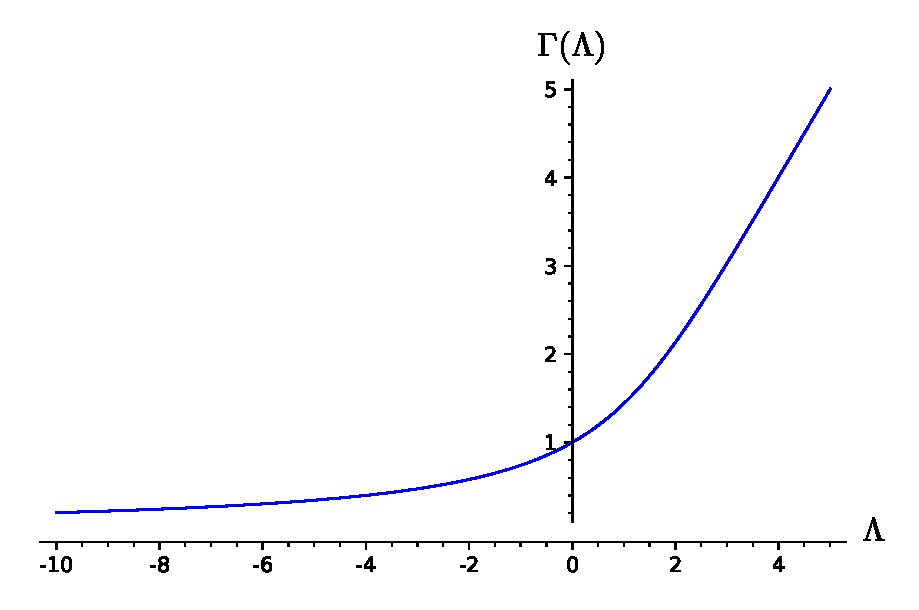
\includegraphics[width=0.5\textwidth]{gamma.eps}
\caption{Rescaled sticking term $\Gamma = (3L/l) \, \gamma$ as a function of rescaled biasing parameter $\Lambda = (L v_0/3) \, s$.}
\label{Gamma}
\end{figure}

%%%%%%%%%%%%%%
% REFERENCES %
%%%%%%%%%%%%%%

\bibliographystyle{alpha}
{\renewcommand{\bibname}{References}\bibliography{ref}}

\end{document}
